\documentclass[a4paper,14pt]{extarticle}

% Russian-specific packeges
%--------------------------------
\usepackage[T2A]{fontenc}
\usepackage[utf8]{inputenc}
\usepackage[russian]{babel}
%--------------------------------
\usepackage{csquotes}
\usepackage{hyphenat}
\usepackage{subcaption}

\usepackage{biblatex} %Imports biblatex package
\addbibresource{ref.bib} %Import the bibliography file

\usepackage{amsmath,amssymb}
\usepackage{indentfirst}
\usepackage{graphicx}

\usepackage[left=3cm, right=1.5cm, top=2cm, bottom=2cm]{geometry} % Меняем поля страницы

\graphicspath{ {diploma_pictures} }

\usepackage{physics}

\linespread{1.3}



\begin{document}
    \thispagestyle{empty}
    \begin{titlepage}
    \small
    \begin{center}
    ФЕДЕРАЛЬНОЕ ГОСУДАРСТВЕННОЕ БЮДЖЕТНОЕ ОБРАЗОВАТЕЛЬНОЕ
    УЧРЕЖДЕНИЕ ВЫСШЕГО ОБРАЗОВАНИЯ \\
    «МОСКОВСКИЙ ГОСУДАРСТВЕННЫЙ УНИВЕРСИТЕТ\\
    имени М.В. ЛОМОНОСОВА»
    \vspace{0.5cm}

    ФИЗИЧЕСКИЙ ФАКУЛЬТЕТ\\
    \vspace{0.5cm}
    КАФЕДРА КВАНТОВОЙ ТЕОРИИ И ФИЗИКИ ВЫСОКИХ ЭНЕРГИЙ\\

    \vspace{0.5cm}
    БАКАЛАВРСКАЯ РАБОТА \\
    \vspace{3cm}

    \textbf{<<Поиск возможностей повышения чувствительности экспериментального исследования спектра бета-распада молекулярного трития к оценке эффективной массы электронного антинейтрино.>>}


    \end{center}


    \begin{flushright}
    \vspace{3cm}

    Выполнил студент \\
    408 группы\\

    Зубрилин Кирилл Васильевич \\

    \underline{\hspace{3cm}}\\

    \vspace{0.5cm}

    Научный руководитель:\\
    д.ф.\--м.н. Свешников Константин Алексеевич \\
    \underline{\hspace{3cm}}\\
     
    \vspace{0.5cm}

    Научный консультант:\\
    к.ф.\--м.н. Титов Никита Андреевич \\
    
    \end{flushright}

    %\vspace{1cm}
    \begin{flushleft}
    Допущена к защите \\
    Зав. кафедрой \underline{\hspace{3cm}} \\
    \end{flushleft}
    \begin{center}
    \vspace{1.5cm}
    \small МОСКВА \\ \number\year\normalsize
    \end{center}
    \end{titlepage}

    \tableofcontents
    \setcounter{page}{2}
    \newpage
    \section{Введение}

    %===========================================================================================
    Нейтрино являются весьма особенными для науки частицами, которые снова и снова 
    приводили к неожиданным и невероятным открытиям, ряд из которых отмечен Нобелевскими 
    премиями. Нейтрино были теоретически введены в 1930 году Паули для выполнения закона сохранения 
    энергии-импульса, а их первое экспериментальное обнаружение состоялось в 1956 году 
    группой Рейнеса и Коуэна на реакторе электростанции Savannah River. Позже оказалось, что существует три аромата нейтрино,
    что снова стало важным открытием. Затем были зарегистрированы осцилляции солнечных 
    нейтрино по пути их распространения к Земле, что является квантовомеханическим эффектом,
    обычно проявляющимся лишь в атомных масштабах. Было обнаружено, что нейтрино имеют 
    очень маленькую массу, что до сих пор является единственным значимым свидетельством
    существования физики элементарных частиц за пределами Стандартной модели. Есть множество других областей, где уже признано, 
    что нейтрино играют важную роль, но есть очень серьезные поводы полагать, что в будущем 
    могут появиться еще более удивительные результаты. Нейтрино — это безмассовые частицы в 
    Стандартной модели. Прямое расширение СМ для введения масс нейтрино, аналогичных массам 
    заряженных лептонов, заключается в добавлении правых (синглетных) нейтринных полей; в этом 
    случае  взаимодействия Юкавы будут свидетельствовать о наличии дираковских масс нейтрино 
    после нарушения электрослабой симметрии. Однако это предположение не считается удовлетворительным 
    сообществом теории нейтрино по двум причинам: а) не объясняет, почему абсолютная шкала 
    массы нейтрино по крайней мере в миллион раз меньше, чем массы других фермионов СМ, и 
    б) симметрии СМ не запрещают другие, так называемые Массовые члены Майораны для недавно 
    введенных правых полей нейтрино. Эти массы не ограничены сверху средним значением вакуума 
    Хиггса и, следовательно, должны принимать много большие значения, чем масса t-кварка. 
    Принимая во внимание массовые члены Майораны, мы получим эффективные массы легких майорановских 
    нейтрино в абсолютной шкале масс нейтрино $m_{\nu} \simeq m^2_D/M_R$; здесь $m_{D}$ и $M_R \geq 10^{14}$ ГэВ 
    величины электрослабого нарушения симметрии и тяжелых майорановских нейтрино соотвественно. 
    Этот механизм установлен как механизм качелей типа I \cite{minkowski} 
    \cite{https://doi.org/10.48550/arxiv.1306.4669}; это интересно, так как дает описание 
    малости массы нейтрино, имеет потенциальную связь с лептогенезом и может даже подразумевать 
    отношение к шкале, объединяющей электрослабое и сильное взаимодействия. Тогда массы легких 
    нейтрино появляются как собственные значения массовой матрицы Майорана, а матрица 
    Понтекорво-Маки-Накагава-Саката (далее ПМНС) U получается из относительного вращения полей 
    левых заряженных лептонов и нейтрино (с которыми связан заряженный ток).
    
    Вспомним, что абсолютные массы нейтрино появляются в теории как собственные состояния матрицы 
    эффективных масс легких нейтрино. Хотя эксперименты с нейтринными осцилляциями способны измерять 
    расщепление квадрата массы среди них и даже упорядочение масс, они не могут дать абсолютную 
    шкалу масс нейтрино. Осцилляции нейтрино дают нижнюю оценку суммы масс нейтрино 0,06 эВ и 0,10 эВ 
    для нормального и обратного порядков соответственно, в то время как текущие верхние границы, полученные 
    различными методами, $\simeq$ 1 эВ. Если сумма масс нейтрино близка к нижней границе, мы говорим 
    об иерархической схеме, где масса легкого нейтрино ближе к нулю по сравнению с расщеплениями масс. 
    Если она близка к верхней границе, то речь уже идет о вырожденных массах нейтрино, поскольку расщепления 
    $|\Delta m^2| \ll m^2 $ малы по сравнению с массами. Порядок масс нейтрино и масштаб шкалы являются
    важными параметрами для теоретических моделей, потому что устройство аромата в лагранжиане, описывающем 
    массу нейтрино будет сильно различаться в нормальном иерархическом, обратном иерархическом и вырожденном случаях. 
    
    В значительной степени независимым способом получить абсолютную шкалу масс нейтрино 
    являются точные кинематические эксперименты по изучению слабых взаимодействий. Сегодня 
    основные усилия направлены на исследования процессов в двух нуклидах: бета-распад трития ($^{3}$H) и 
    захват электрона гольмием ($^{163}$Ho). Что интересно, данные методы позволяют независимо 
    получить массы электронных нейтрино и антинейтрино, которые должны быть равны при CPT 
    инвариантности. Особенность данных методов состоит в том, что напрямую измеряются квадраты
    масс нейтрино, что накладывает некоторые трудности в получении дополнительного порядка
    точности по отношению непосредственно к массе. 
    
    Для тритиевых экспериментов используются спектрометры с электростатистическим замедлением
    для получения максимального углового разрешения (так называемые MAC-E фильтры) \cite{lobashev} \cite{picard}.
    Проект КАТРИН в полной мере использует данную технологию, что на сегодняшний день позволило
    получить значение верхней границы массы нейтрино 0.8 эВ (при 90\% доверительном уровне) \cite{aker}.
    КАТРИН продолжит набор статистики для достижения заложенной чувствительности на уровне
    0.2 эВ.
    
    В данной же работе будут исследоваться способы повышения чувстиветельности исследования к 
    оценке массы электронного антинейтрино.
     

    %===========================================================================================


    %===========================================================================================
    \newpage
    \section{Обзор задачи}
    \subsection{Устройство спектрометра}
    Высокая чувствительность экспериментов по массе нейтрино в Троицке и Майнце обусловлена
    новым типом спектрометра, так называемым MAC-E (магнитным адиабатическим коллимационным
    + электростатическим) фильтром. Впервые этот новый тип спектрометра был предложен
    в \cite{Beamson_1980}. Позднее этот метод был переизобретен специально для поиска массы электронного
    нейтрино в Троицке и Майнце \cite{lobashev} \cite{picard}, независимо друг от друга. Он сочетает в 
    себе высокие светимость и энергетическое разрешение, необходимые характеристики для измерения 
    массы нейтрино в конечной области спектра $\beta$-распада.
    
    Основные характеристики MAC-E-фильтра показаны на рис. \ref{fig:spectrometer}(a) \cite{design_report}. 
    Два сверхпроводящих соленоида создают направляющее магнитное поле. Электроны, запускаемые 
    из источника трития в левом соленоиде в переднюю полусферу, направляются при
    циклотронном движении вокруг линий магнитного поля в спектрометр, что позволяет достичь
    телесного угла прием влоть до 2$\pi$. На их пути в центр спектрометра
    магнитное поле B падает на несколько порядков. Следовательно, магнитный градиент
    преобразует большую часть энергии циклотрона $E_\perp$ в продольное движение. Это
    показано на рис. \ref{fig:spectrometer}(б) вектором импульса. Из-за медленно меняющегося магнитного 
    поля импульс преобразуется адиабатически, поэтому магнитный момент $\mu$ остается постоянным:
    
    \begin{equation}\label{adiabat}
        \mu = \frac{E_\perp}{B} = const.
    \end{equation}
    
    Это преобразование можно резюмировать следующим образом: электроны, изотропно испускаемые
    источником, преобразуются в широкий пучок электронов, летящих почти параллельно линиям
    магнитного поля.
    
    \begin{figure}
        \center
        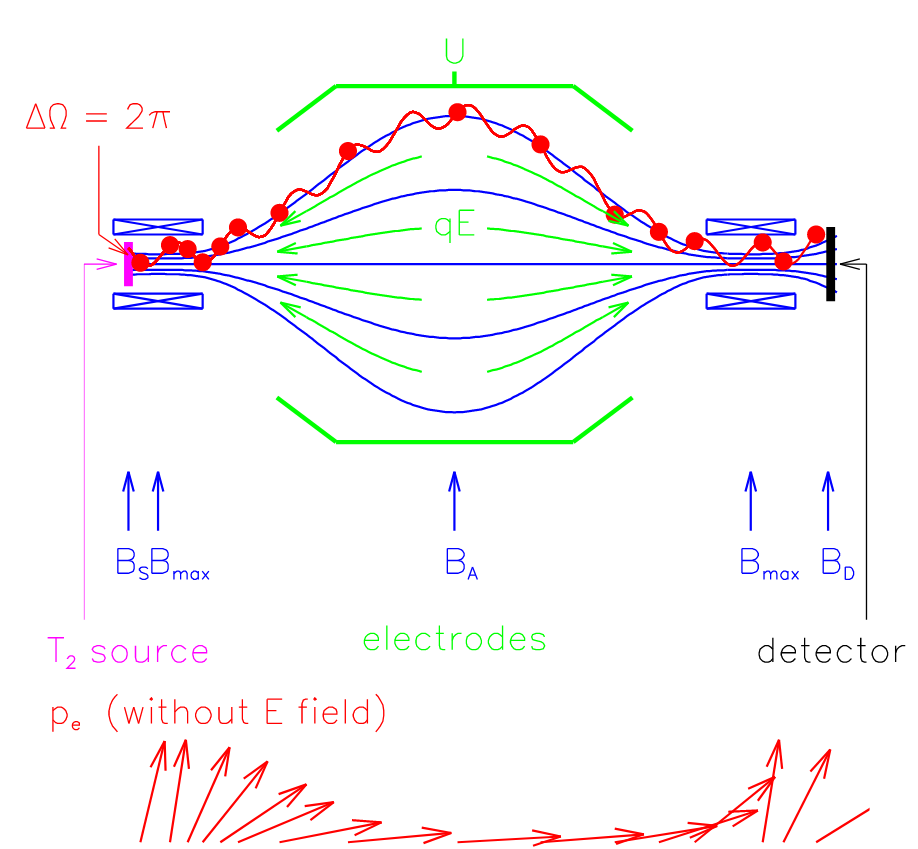
\includegraphics[width=0.6\textwidth]{spectrometer.png}
        \captionsetup{width=0.8\textwidth}
        \caption{Принципиальная схема MAC-E фильтра. (а) Экспериментальная установка, (б) Преобразование вектора импульса, обусловленное адиабатическим инвариантом $\mu$.}
        \label{fig:spectrometer}
    \end{figure}
    
    Получившийся параллельный пучок электронов летит против градиента электростатического потенциала, образованного
    одним или несколькими цилиндрическими электродами. Все электроны с энергией, достаточной для прохождения
    электростатического барьера, ускоряются и коллимируются на детекторе, остальные же отражаются.
    Таким образом спектрометр действует как интегрирующий высокоэнергетический фильтр. Из уравнения (\ref{adiabat})
    непосредственно следует, что относительная резкость $\Delta E/E$ этого фильтра определяется только соотношением
    минимального магнитного поля $B_A$ в центральной плоскости и максимального магнитного поля
    $B_{max}$ между источником электронов и спектрометром:
    
    \begin{equation}
        \label{form2}
        \frac{\Delta E}{E} = \frac{B_A}{B_{max}}
    \end{equation}
    
    Чтобы подавить электроны, которые имеют очень длинный путь внутри источника трития
    и, следовательно, обладают высокой вероятностью рассеяния, источник электронов помещается в
    магнитное поле $B_S$, которое меньше максимального магнитного поля $B_{max}$.
    Это ограничивает максимально допустимый начальный угол электронов $\theta_{max}$ 
    отражающим эффектом магнитного поля:
    
    \begin{equation}
        \label{form3}
        \sin \theta_{max} = \sqrt{\frac{B_S}{B_{max}}}.
    \end{equation}
    
    Из ур. (\ref{adiabat}), (\ref{form2}) и (\ref{form3}) следует, что нормированная функция пропускания MAC-E
    фильтра с задерживающим потенциалом U для изотропного источника электронов с энергией $E$ дается выражением:
    
    \begin{equation}
      T(E,U) = 
      \begin{cases} 
        0 & , E - qU < 0 \\
        \frac{1 - \sqrt{1-\frac{E-qU}{E} \frac{B_{S}}{B_{A}}}}{1 - \sqrt{1-\frac{\Delta E}{E}\frac{B_{S}}{B_{A}}}} & , 0 \leq E-qU \leq \Delta E \\
        1 & , E - qU > \Delta E
      \end{cases}
    \end{equation}
    
    \noindent где $q$ - заряд электрона.
    
    
    
    \subsection{Расчет спектра}
    Для определения массы нейтрино необходимо сопоставить экспериментальные данные
    с теоретическим предсказанием, полученным с помощью аналитической формулы $\beta$-распада
    и экспериментальной функции отклика, описанными ниже.
    
    Теоретический спектр $R(qU,r)$ задается суммой свёртки дифференциального спектра $\beta$-распада $R_{\beta}(E)$ 
    с экспериментальной функцией отклика $f(E,qU,R)$ и фона $R_{bg}(qU,r)$:
    \begin{equation}
      R(qU,r)=A_s N_T \int_{qU}^{E_0} R_{\beta}(E)f(E,qU,R)dE + R_{bg}(qU,r).
    \end{equation}
    
    Здесь $N_T$ - нормировочная константа сигнала, зависящая от числа атомов трития в источнике, максимального угла
    раскрытия и коэффициента детектирования. $A_s \approx 1$ - дополнительный нормировочный коэффициент, используемый
    как свободный параметр при фитировании. Дифференциальный спектр $\beta$-распада берется из теории Ферми и описывается
    формулой:
    
    \begin{multline}
        R_{\beta}(E) = \frac{G_F^2 \cos^2 \Theta_C}{2 \pi^3} |M_{nucl}|^2 F(E, Z'=2) \cdot \\
        (E + m_e) \sqrt{(E+m_e)^2-m_e^2} \cdot \\
        \displaystyle\sum_f \zeta_f \varepsilon_f(E) \sqrt{\varepsilon_f(E)^2-m_{\nu}^2} \Theta(\varepsilon_f(E)-m_{\nu}),
    \end{multline}
    
    \noindent где $G_F$ - константа Ферми, $\cos^2 \Theta_C$ - угол Кабиббо, $|M_{nucl}|^2$ - независящий от энергии матричный
    элемент, а $F(E, Z'=2)$ - функция Ферми. $\varepsilon_f(E) = E_0 - V_f - E$, где $E_0$ - максимальная кинетическая
    энергия электрона для безмассового нейтрино, $V_f$ описывает спектр возбужденных состояний дочернего молекулярного иона, которые распределены с
    вероятностями $\zeta_f$, $E$ и $m_e$ - кинетическая энергия и масса электрона соответственно.
    
    Экспериментальная функция отклика
    
    \begin{equation}
      f(E-qU) = \int_0^{E-qU} \int_0^{\theta_{max}} \mathcal T(E - \varepsilon, \theta, U) \sin\theta \\
      \cdot \displaystyle\sum_s P_s(\theta)f_s(\varepsilon) d\theta d\varepsilon
    \end{equation}
    
    \noindent выражает вероятноять электрона с начальной энергией $E$ достигнуть детектора. Она содержит функцию 
    пропускания спектрометра $\mathcal T(E - \varepsilon, \theta, U)$ и энергетические потери электрона
    $\varepsilon$, вызванные неупругими столкновениями с молекулами трития в источнике. Потери энергии, вызванные
    рассеянием, описываются как произведение вероятности s-кратного рассеяния $P_s(\theta)$, которая зависит от пути 
    пройденного через источник и, как следствие, угла падения $\theta$, и функции энергетических потерь 
    $f_s(\varepsilon)$ для числа рассеяний s. Функция потерь определяется экспериментально с помощью электронной
    пушки, установленной у входа в источник.
    
    Интеграл от передаточной функции для изотропного источника электронов дается следующей формулой: 
      
    \begin{align}
      T(E,U) = \int_0^{\theta_{max}} \mathcal T(E, \theta, U) \cdot \sin \theta \: \mathrm d \theta = \\
      \begin{cases} 
        0 & , \epsilon < 0 \\
        1 - \sqrt{1-\frac{E-qU}{E} \frac{B_{source}}{B_{ana}} \frac{2}{\gamma + 1}} & , 0 \leq E-qU \leq \Delta E \\
        1 - \sqrt{1-\frac{B_{source}}{B_{max}}} & , E - qU > \Delta E
      \end{cases}
    \end{align}
    
    Он определяется магнитным полем в начальной позиции электрона $B_{source}$, максимумом поля в луче $B_{max}$
    и величиной магнитного поля в анализирующей плоскости спектрометра $B_{source}$.
    
    

    %===========================================================================================
    
    \newpage
    \section{Основная часть}
    
    %===========================================================================================


    %===========================================================================================    
    \section{Выводы}
    
    \section{Заключение}
    
    \newpage
    \newrefcontext[sorting=none]
    \printbibliography[heading=bibnumbered]

\end{document}
